\subsection{Разработка интерфейса взаимодействия}

Графический интерфейс пользователя, согласно выбору архитектуры клиент-сервер, основывается на технологии HTML + CSS + JavaScript с использованием Ajax запросов. 

\subsubsection{Разработка графа диалога}

Разработаем верхний уровень графа диалога с пользователем:
\begin{itemize}
\item \textbf{Главный экран} -- должен содержать элементы интерфейса для наиболее часто используемых функций АИС. Так как основной функцией АИС является поиск по новостным документам, то главный экран содержит рубрикатор, форму ввода поискового запроса и результат выполнения поискового запроса.
\item \textbf{Экран импорта} -- должен содержать элементы интерфейса для добавления документов в систему, а именно: форму ручного ввода, импорт архива документов и управление автоматизированным импортом документов из папки импорта.
\item \textbf{Экран экспорта} -- должен содержать элементы интерфейса для экспорта документов из системы.
\item \textbf{Экран управления} -- должен содержать элементы интерфейса для управления длительными операциями над индексом документов, над рубрикатором и другими действиями с предоставлением информации о прогрессе операции.
\item \textbf{Экран настроек} -- должен содержать элементы интерфейса для изменения и просмотра пользовательских настроек системы.
\item \textbf{Экран прогноза} -- должен содержать элементы интерфейса для отображения графиков активности новостных потоков, графики прогноза их активности, оценку качества прогноза и результирующую аналитическую функцию прогноза.
\end{itemize}

Обобщенный граф диалога представлен на рисунке~\ref{figure:dialog_generic}.

\clearpage
\begin{figure}[h!]
\centering
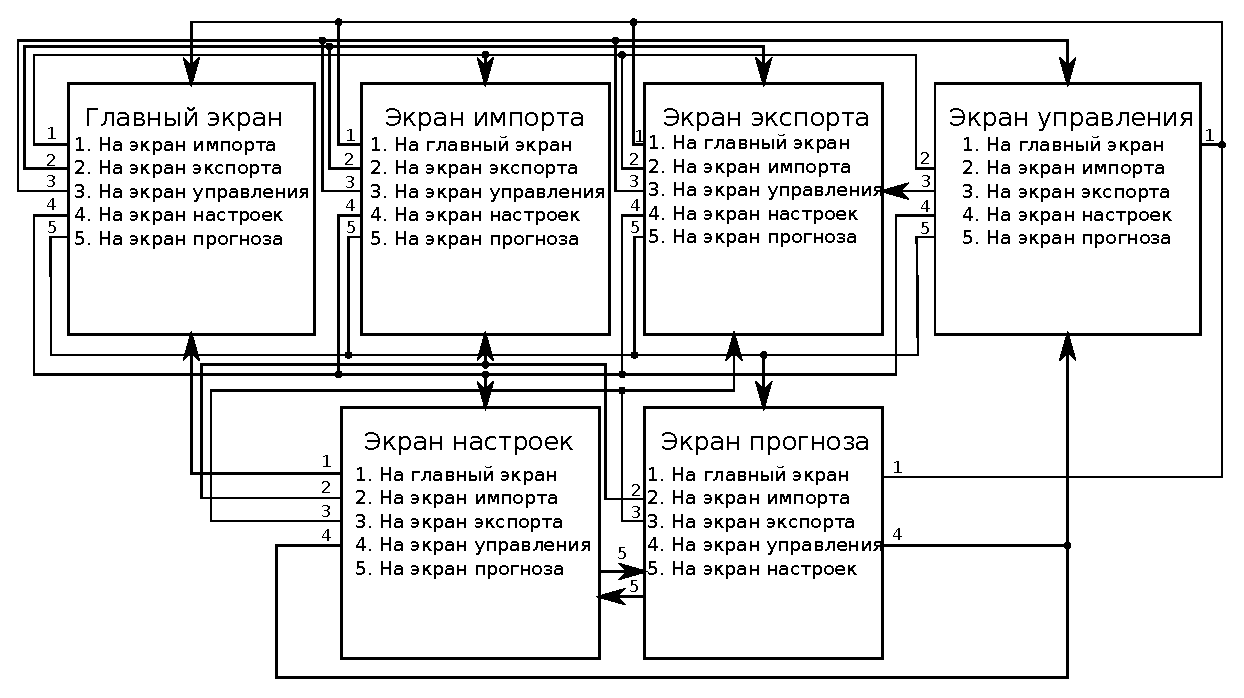
\includegraphics[angle=90,origin=c]{technology/dialog_generic}
\caption{Обобщенный граф диалога взаимодействия с пользователем}
\label{figure:dialog_generic}
\end{figure}

\subsubsection{Разработка экранных форм}



\subsection{Описание экранных форм}